\chapter[Localization and Object Detection]{Beyond image classification: Localization and Object Detection}

\begin{quotation}
    \noindent
    \textsf{In this chapter we will see other Computer Vision tasks which goes beyond classification: we are talking about \textit{localization} (the task of localizing a given object by using a bounding box into an image) and \textit{object detection} (the task of localizing multiple object within an image with their bounding boxes).
    }
\end{quotation}

\section{Classification with localization}
Here we are talking about of an extension of the concepts we have presented for classification in order to give as output of the prediction for an object of a given class a \textbf{bounding box} for the object itself in term of box coordinates. This is of big practical interest: Autonomous driving, Industry 4.0, Pedestrian detection and so on.\\
Let us say that our final objective is, given an image, detecting multiple object inside it with both a \textbf{confidence score} and a \textbf{bounding box}. However in order to better and slightly understand, here we focus at first on a simpler task: \textbf{there is a single object to detect} within the image, the difference now is that we want to find the bounding box. How can we do it? It is quite "simple"! \\
Let us suppose that we have our CNN for the classification of five class of objects, say, \textit{pedestrians, car, motorcycle, background}. In the last part of the network, we have some fully connected layers, that at the end will say by using a softmax some confidence scores. It is sufficient to introduce some new \textbf{numbers} for the network to learn which are related to the object bounding box (these can be the coordinate of the top-left most point and width/height of the box itself). 

\begin{figure}
    \centering
    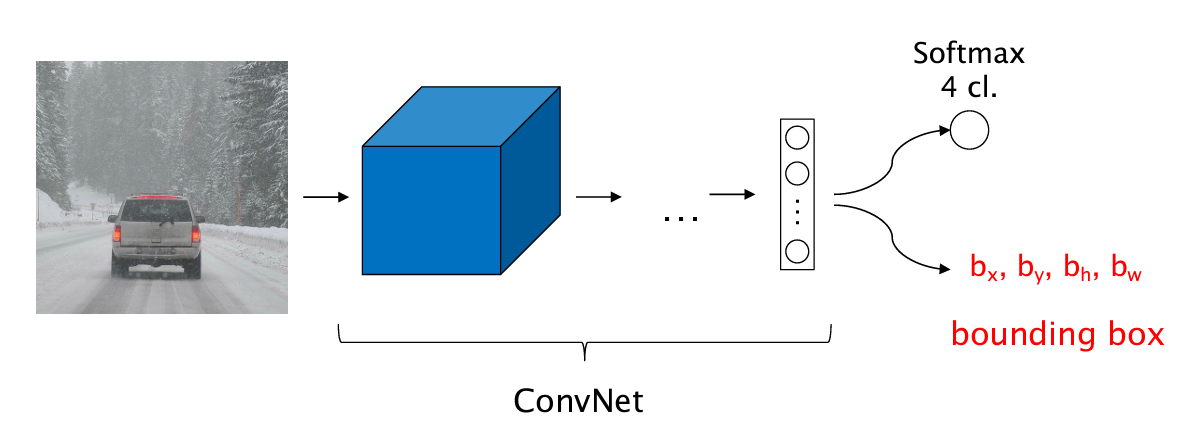
\includegraphics[scale=0.5]{img/CNN_localization.png}
    \caption{Classification + localization}
\end{figure}

The predicted output $\hat{y}$ of the ConvNet in this case is made up of $C+5$ numbers where $C$ is the number of classes. 
For example if we have 3 classes $y$ (and then $\hat{y}$) is like: 

\begin{multicols}{2}
    \begin{equation}\label{eq:obj_label}
        y=\begin{bmatrix}
            p_c\\b_x\\b_y\\b_h\\b_w\\c_1\\c_2\\c_3
        \end{bmatrix}=\begin{bmatrix}
            0.95\\0.5\\0.9\\0.3\\0.5\\0\\1\\0
        \end{bmatrix}
    \end{equation}
    \newcolumn

    \noindent
    The number $p_c$ is \textit{confidence level} used to indicate whether in the image is present or not an object of any class; this is followed by four numbers the normalized coordinates of the top left corner (or the center) of the bounding box ($b_x,b_y$) and its normalized width and height ($b_h, b_w$); the last three numbers tells us (using a one-hot encoding fashion) what is the class to which the localized object is associated.
\end{multicols}
One possible choice for the \textit{loss function} is the following: 
\begin{equation}
    \text{Loss}(\hat{y}, y)=
    \begin{cases}
        \sum_{i=0}^{8} {(\hat{y}_i-y_i)^2}&\text{if} \ y_1=1\\
        (y_1-\hat{y_1})^2&\text{if} \ y_1=0
    \end{cases}
\end{equation}

\noindent 
In order to give some \emph{take away} information, we can say that the localization task can be performed using the architectures of CNN we have already seen with the only difference we are asking to the network to learn some other additive information related to the bounding box of the (potentially) classified object. To tell the truth we can do also other things: for example we can train the network so that it can detect \textit{joint positions} and \textit{landmark}.This is the right moment to highlight the fact that here we are combining two different but integrated tasks: \textbf{\underline{classification} of images} and \textbf{\underline{regression} of bounding boxes}.
Now, what is the drawback? Often the labeling of the samples must be done "by hand" using some specific tools. As you can imagine, since a DNN needs a large amount of data this task is not so easy.

\section{Object detection}
Are we able to perform classification using DNN and the added information we have just introduced? Practically speaking, yes, but in what sense? Using one of the most famous computer science paradigms: \textit{divide-et-impera}.\\
Let us suppose our (fine-tuned) ConvNet is trained for \textit{localizing cars} and we want to detect within an image \textbf{multiple cars}. We can split the input image in a set of \textbf{crops} using a \textbf{sliding window} with certain dimensions. At the end of the day we have that some crops are containing the localized cars and we are done! The task of detecting multiple object within an image has been carried out by blindly applying the well-known techniques. Several problem occurs: what is the ideal dimension for the sliding window? What if I use a stride? Is it better, worse? More than this, this solution \textbf{does not scale} and cannot be use for large scale and real time object detection: identical computations are repeated over and over without reusing them! 

\subsection{OverFeat: a fully Convolutional Architecture}
We know from the previous chapter that a generic ConvNet in its final part has a \textbf{classificator} which is constituted by several fully connected layers, we have seen also that different architectures have different \textit{dense} layers with several units. By using 1x1 convolutions we can turn replace such layers with convolutional ones, clearly there is not an equivalence, but the architecture use convolutions \textit{end-to-end} from the input to the output.

\begin{figure}
    \centering
    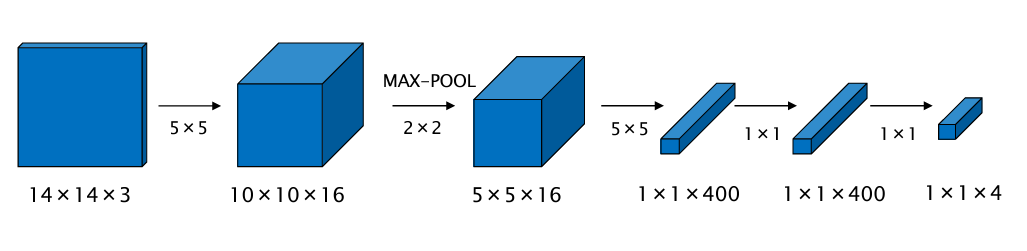
\includegraphics[scale=0.6]{img/FCN.png}
    \caption{Fully Convolutional network}
\end{figure}

This idea is used in \cite{sermanet_overfeat_2014} as fundamental idea to implement a network that in an integrated way perform three tasks of increasing difficulty: \textit{recognition/classification}, \textit{localization} and \textit{detection}. The main idea is \textbf{using the convolutional network} in a \textit{sliding window fashion}. When convolutions are applied from the input to the output make the network producing a \textbf{map of class predictions} with one \textbf{spatial location} for each \textit{window} (field of view) of the input.

\begin{figure}[h]\label{fig: OverFeat_1}
    \centering
    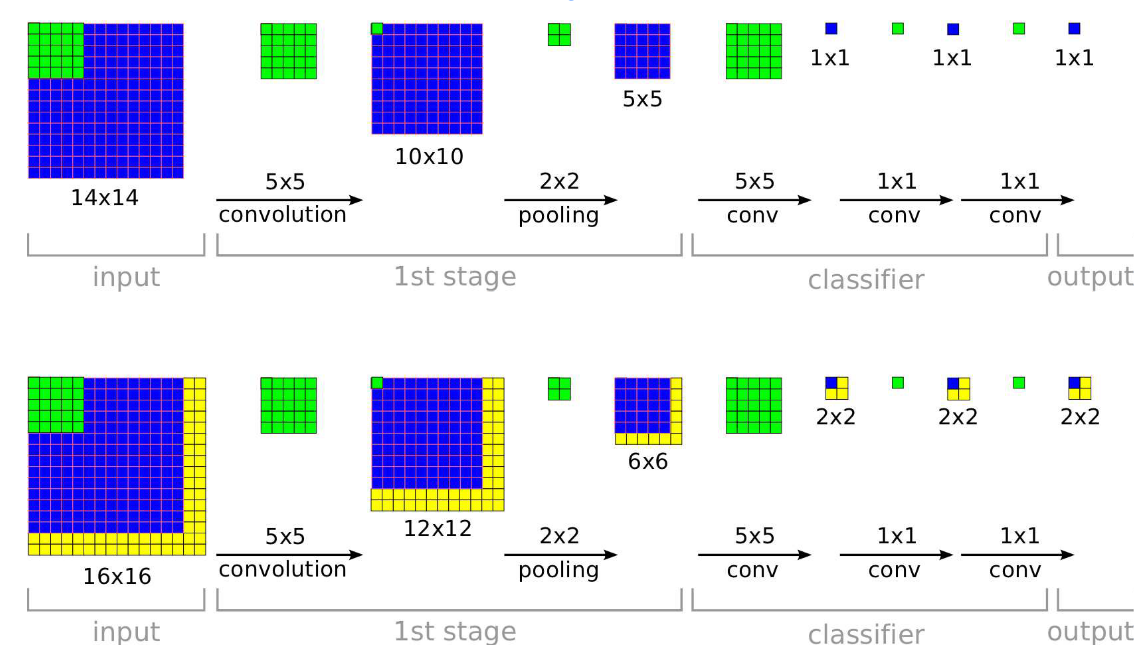
\includegraphics[scale=0.5]{img/OverFeat.png}
    \caption{Convolutions and produced output maps}
\end{figure}

\noindent
In the context of DNN the concept of \textit{field of view} or \textbf{receptive field} is central. In particular it is defined as \textbf{the size of the region of the input that produces a feature} at a certain convolutional layer, since it is well known that by construction each one of the feature in the intermediate level depends only from a part of the input.

\begin{figure}[h]
    \centering
    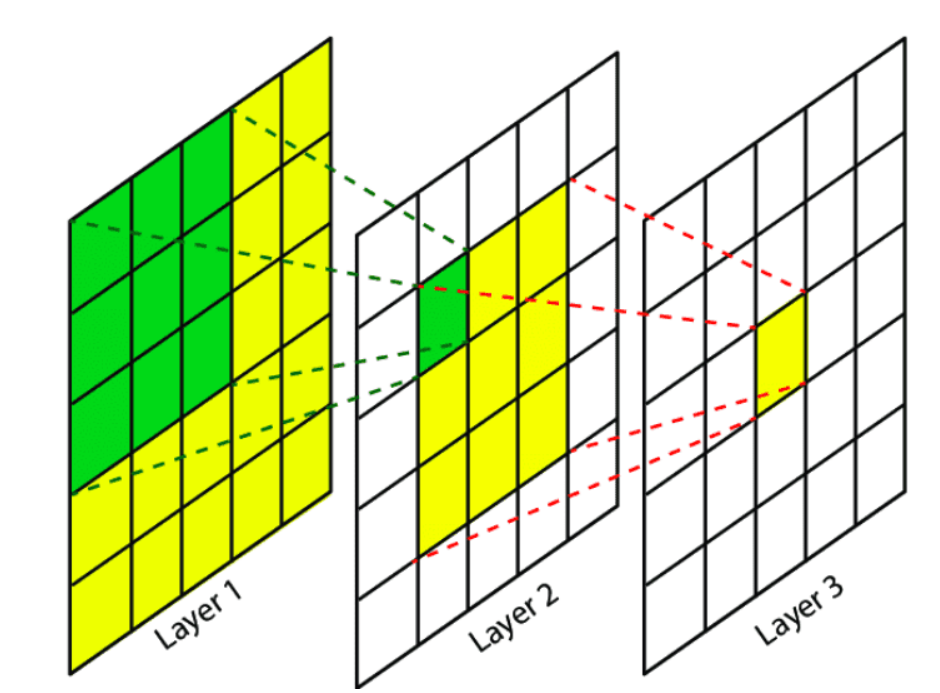
\includegraphics[scale=0.3]{img/ReceptiveFields.png}
    \caption{Receptive field (field of view)}
\end{figure}

In the case of \textit{OverFeat} \cite{sermanet_overfeat_2014} the dimension of the receptive field, that play effectively the role of sliding window, is strongly connected to to the dimensions of convolutional and pooling filters. In the specific analysed case the dimension of the sliding window (in turn \textit{receptive field}) is $14\times14$. The output is a map $2\times2\times4$ that are nothing but the information in (\ref{eq:obj_label}) for each one of the four subregions of our image\footnote{
    Note that we have potentially: identified multiple objects while classifying them and providing a bounding box. We assessed all of the three tasks: classification, localization and detection.
}. Clearly if we change the parameters of the filters (at different stages) also the receptive field is different. The figure \ref{fig: OverFeat_1} shows the results after the convolutions starting from a $14\times14\times3$ image and for a $16\times16\times3$, the yellow region is associated to the added computation with the increased input size, this is for underlining again the fact that using convolutions there are a lot of shared computations. We have cited \cite{sermanet_overfeat_2014} in order to do a first step toward the more sophisticate techniques for object detection. The paper explain very well what is the manner by which we are getting rid of all the useless bounding box, you can refer to it for further details. However, briefly speaking,  differently from the naive approach that compute an entire pipeline for each one of the analyzed crop, here there is a sharing of computations among overlapped regions.

\subsection{Region Proposal: R-CNN}
In the previous chapter we have seen that a first more cleaver approach to object detection is using a fully convolutional network which improves a lot the original sliding window approach, however we can do better. \\
In 2014, in \cite{girshick2014rich} was proposed a new architectures that completely eliminates the sliding window concept since it is inefficient and can produce a large amount of useless information. Such an architecture is made up of \textbf{three modules}: 
\begin{itemize}
    \item The first generates \textbf{region proposals} by using some \textit{proposal methods} such as \textit{Selective Search}\footnote{
        \textbf{Selective Search}, just for give an example, operates by merging or splitting segments of the image based on various image cues like color, texture, and shape to create a diverse set of region proposals.}; a region proposal is a region of the input image which is likely to contain an object of a given class. Before passing to the second stage, each of one of the proposed region is \textbf{warped} in order to make it of suitable dimension for the following stage;  
    \item The \textbf{second module} is a CNN, and in particular AlexNet or VGG-16 fine tuned on the ImageNet dataset. The output of this stage is a \textbf{feature vector} which representing the content of the region.
    \item The \textbf{third stage} is the one in which each feature vector is fed into a machine learning classifier trained on the class of interest (SVM is used).
\end{itemize}

In addition to the classification, of the RoI (Region of Interest) there is a part of the architectures which is devoted to the \textit{regression of the bounding boxes}. In particular for each class there is a trained regressor that refines the initial boxes retrieved by using proposal methods.\\

After having predicted the bounding boxes for each region proposal, \textbf{non-max suppression} (see later) is applied in order to eliminate the 'non-optimal' boxes. In this way the \textbf{final object detection are obtained}.

\begin{figure}
    \centering
    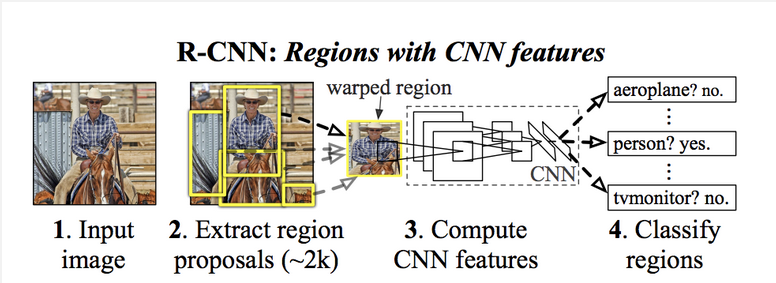
\includegraphics[scale=0.7]{img/R-CNN_1.png}
    \caption{R-CNN structure} 
\end{figure}

\subsubsection{R-CNN features}
Despite R-CNN are a step ahead in the field of Computer Vision, there are some non trivial drawbacks to be taken into account: 
\begin{itemize}
    \itemsep-0.3em
    \item Training is very slow (84h), requires a lot of space on the disk;
    \item Making a prediction is very slow, 47s for image (using as backbone\footnote{
        In the field of Computer Vision and DNN, \textbf{backbone architecture} is generally, the term backbone refers to the feature-extracting network that processes input data into a certain feature representation.
    } architecture VGG-16)
\end{itemize}

\section{Fast R-CNN}
We have seen that in R-CNN the main problem is that the \textbf{training is a multi-stage pipeline}, moreover it is expensive and it requires long time in order to correctly perform detection. In order to solve such problems, in \cite{DBLP:journals/corr/Girshick15} \citeauthor{DBLP:journals/corr/Girshick15} proposes a new method which has several advantages: 
\begin{itemize}
    \itemsep-0.3em 
    \item Higher performances with respect to R-CNN;
    \item The training is done in a \textbf{single stage} while using a \textbf{multi-task} loss.
\end{itemize}
A \textit{Fast R-CNN} network takes as input an \textbf{entire image} from which is extracted a common feature map and a set of \textbf{object proposal}. Then, for each object proposal a \textit{Region of Interest (RoI)} pooling layer extracts a fixed length feature vector from the feature map. \underline{Each feature vector} is fed up into a sequence of fully connected layers that finally branch into two output layers: one producing a softmax probability for the $K$ classes plus one \textit{catch-all} "background" class; the other is producing four real-valued numbers related to the \textbf{refined bounding-box} for that RoI. Note that the region proposals are obtained via non-neural methods, moreover the architecture related to the neural part is trained e2e (end-to-end).
The following shows and summarizes the main features of \textit{Fast R-CNN}:

\begin{figure}[h]
    \centering
    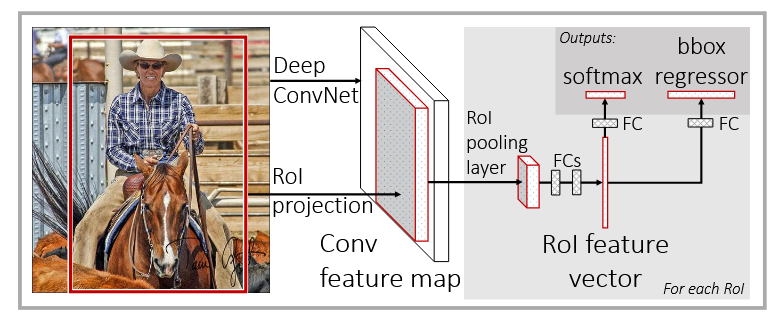
\includegraphics[scale=0.5]{img/FRCNN.png}
    \caption{\textbf{Fast R-CNN architecture}. An input image and multiple region of interest (RoIs) are input into a Fully Convolutional Newtork. Each RoI is pooled into a fixed-size feature map and then mapped to a \textit{feature vector} by fully connected layers} 
\end{figure}
How it is showed in the following histograms the bottleneck of Fast R-CNN is the RoI generation, without it we achieve a \textit{near real-time} object detection.


\begin{figure}
    \centering
    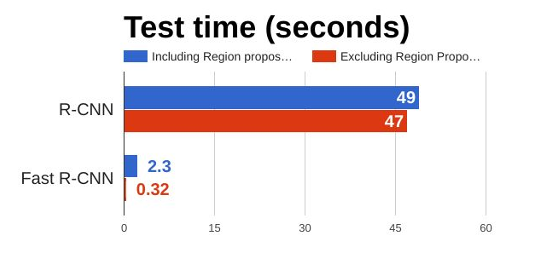
\includegraphics[scale=0.7]{img/FRCNN_histogram.png}
    \caption{R-CNN and Fast R-CNN compared wrt Test time}
\end{figure}

\citeauthor{DBLP:journals/corr/RenHG015} (see \cite{DBLP:journals/corr/RenHG015}) solved this problem by introducing the so-called \textit{region proposal network} that is completely based on ConvNets.

\section{Faster CNN}
Such an object detection system, called \textbf{Faster R-CNN} is composed of two modules related two networks which are trained jointly. The first is a \textit{deep fully convolutional network} that proposes regions and works in a sliding-window fashion, the second module is the \textbf{Fast R-CNN} detector that substancially uses the proposed regions. In practice, the RPN (Region Proposal Netwoek) tells the Fast R-CNN where to look. The architecture of the network is presented in the figure that follows: 

\begin{multicols}{2}
    \begin{center}
        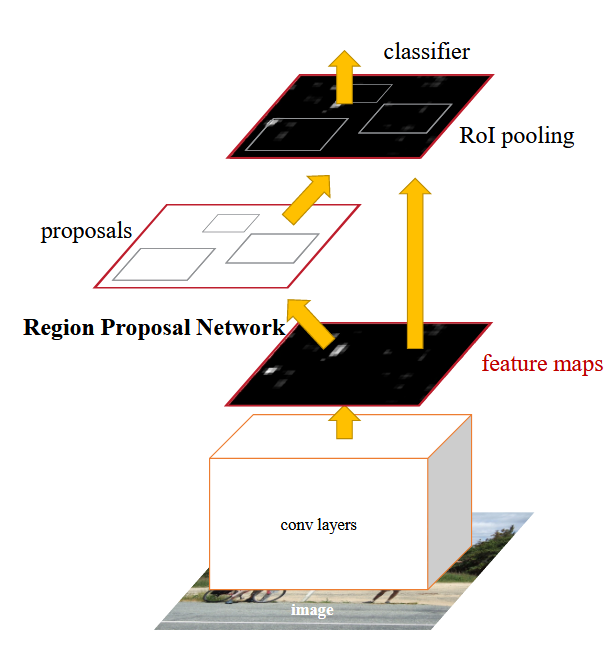
\includegraphics[scale=0.5]{img/FasterRCNN-.png}
    \end{center}
    \noindent
How it is written in the paper: \begin{quotation}
    \noindent
    \emph{"Faster R-CNN is a single, unified network for object detection. The RPN module serves as the 'attention' of this unified network." 
    }
\end{quotation}
Keep in mind that our goal is to share computation with a Fast R-CNN object detection network, both RPN and Fast R-CNN share common convolutional layers constituting the \textbf{backbone architecture}. Another detail is that for each region proposal several bounding boxes are predicted simultaneously. In conclusion the loss function is something like:
\begin{equation}
    L = \alpha{L_{cls}} + \beta {L_{reg}}
\end{equation}
where $L_{reg}$ is the contribution for bounding boxes prediction, while $L_{cls}$ is the contribution for the classification. 
\end{multicols}


\begin{table}
    \centering
    \begin{tabular}{@{}l l l @{}}
    \toprule
    \textbf{Aspect}           & \textbf{Fast R-CNN}                      & \textbf{Faster R-CNN}                  \\ \midrule
    \textbf{Region Proposal}  & External (e.g., Selective Search)        & Integrated RPN                         \\
    \midrule 
    \textbf{Speed}            & Slower                                   & Faster                                 \\  \midrule
    \textbf{Architecture}     & Two-stage, with separate proposals       & Unified, shared layers with RPN        \\ \midrule
    \textbf{Training}         & Partially end-to-end                     & Fully end-to-end                       \\ \midrule
    \textbf{Performance}      & Good                                     & Better (accuracy and speed)            \\ \bottomrule
    \end{tabular}
    \caption{Comparison of Fast R-CNN and Faster R-CNN}
    \label{tab:comparison}
    \end{table}
\noindent
The \Cref{tab:comparison} shows main differences between \textit{Fast R-CNN} and \textit{Faster R-CNN}.


\section{You Only Look Once (YOLO)}
In this section we introduce YOLO (see \citetitle{redmon2016you} \cite{redmon2016you}) which is a \textbf{single shot method} that \underline{do not use} region proposals, since it performs localization and classification at the same time. YOLO has the following features: 
\begin{enumerate}
    \itemsep-0.3em
    \item In order to handle complexity decomposes the image in a regular grid $S \times S$; 
    \item \textbf{If the center of an object falls into a grid cell, it is responsible for detecting that object}
    \item \underline{Each grid cell} predicts $B$ bounding boxes and confidence scores for those boxes; 
    \item \underline{Each grid cell} also predicts $C$ conditional class probabilities, in particular there is \textbf{one set} of class probabilities, regardless of the number of boxes $B=S\times S$
\end{enumerate}
 
\subsection{Basics for YOLO}
The output label $y$ for the trainng of the model has a shape very similar than the one we have seen in \Cref{eq:obj_label}, clearly it depends also on the number of classes we have.\footnote{
    The most common example when YOLO is cited, is the one with \emph{Pascal VOC} dataset where the output tensor is: $7\times7\times30$ since whe have $S=7$ and $C=20$ with $C$ the number of classes.
}
In order to better understand the main concept behind such a method, we use an example: 

\begin{multicols}{2}
    \begin{center}
        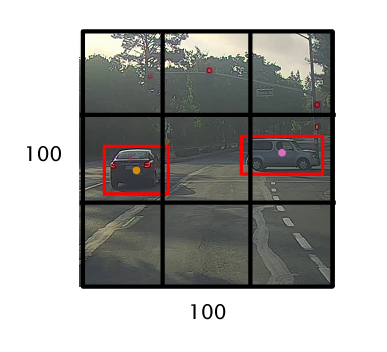
\includegraphics[scale=0.5]{img/YOLO_1.png}
    \end{center}
    \vspace{-0.5cm}
    For sake of simplicity we use a simplified version in which we take a tensor input of $100\times100\times3$. Here $S=3$, $C=3$. Among all the cells of the image what happens is that almost all of them will have $p_c=0$ since no object of the given classes is found. The coordinates of the center are normalized with respect to a certain cell, while width and height can  be for sure greater than 1. Here we assume that a single bounding box per cell is predicted.
\end{multicols}

\subsection{Overlapping objects: introduction of anchors}
\emph{What happens if there is more than one object in a grid cell?} You are supposed to be able to make \textbf{more than one prediction} per cell. The novelty of the anchors have been introduced from YOLOv2. Clearly the dimension of the output and the label used for training grows of a factor equal to the number of anchors. In particular it will be
\begin{equation}
    S\times{S}\times(A\cdot(1+4+C))
\end{equation}
where $A$ is the number of anchors. With the introduction of the anchors \emph{each object in training image is assigned to grid cell that contains object's midpoint and anchor box for the grid cell with highest IoU}. It is remarkable that \textbf{anchor boxes} are human-encoded priors on the size and aspect ratio of the objects. These are tipically defined as a list of pairs (height, width)\footnote{    The anchor boxes are usually determined based on the statistics of the dataset-that is, by analyzing the ground truth bounding boxes and clustering their widths and heights using methods like K-means clustering.
}. The predictions are improved since the bounding boxes are not retrieved from scratch but using prior information.\\
Once the image is passed through the architecture a \textbf{post-processing stage} is required:
\begin{itemize}
    \item For each cell grid, we have some bounding boxes with associated probability.  The first step is getting rid of the low probability predictions (these will be associated to cell in which there are no object to detect), then \textbf{for each class} \underline{non-max suppression} is used.
    \item The selected bounding boxes and associated labels are drawn on the image by using suitable tools/libraries\footnote{
        In particular, \textbf{bounding boxes} are drawn as rectangles using scaled coordinates, \textbf{labels} and \textbf{certainty} scores are shown with a background for ease of reading.
    }.
\end{itemize} 

\begin{figure}
    \centering
    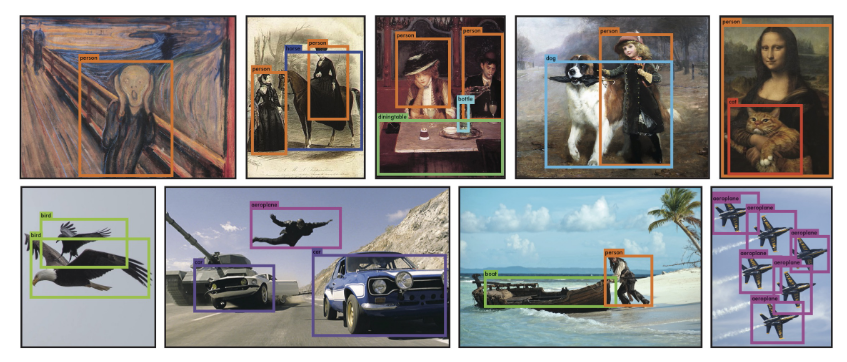
\includegraphics[scale=0.7]{img/YOLO_results.png}
    \caption{YOLO running on sample artwork and natural images from the internet}
\end{figure}

\subsubsection{Scaling Bounding Box Coordinates \small{(Example by ChatGPT)}}

    Let's assume that the bounding box coordinates are given in the original image (e.g., YOLO's default grid size of \( 416 \times 416 \)) and we need to scale them to a new image size (e.g., \( 1000 \times 667 \)).

\noindent
The original coordinates are:
\[
x_{\text{min}} = 116, \quad y_{\text{min}} = 132, \quad x_{\text{max}} = 241, \quad y_{\text{max}} = 340
\]

\noindent
The new image dimensions are \( \text{new\_width} = 1000 \) and \( \text{new\_height} = 667 \).

\noindent
We can scale the coordinates as follows:
\begin{align*}
    x_{\text{min}}' = \frac{x_{\text{min}}}{\text{old\_width}} \times \text{new\_width} \quad 
    y_{\text{min}}' = \frac{y_{\text{min}}}{\text{old\_height}} \times \text{new\_height}\\
    x_{\text{max}}' = \frac{x_{\text{max}}}{\text{old\_width}} \times \text{new\_width} \quad 
    y_{\text{max}}' = \frac{y_{\text{max}}}{\text{old\_height}} \times \text{new\_height}
\end{align*}


\noindent
Substituting the values:

\begin{align*}
    x_{\text{min}}' = \frac{116}{416} \times 1000 = 278.85 \approx 279 \qquad
    y_{\text{min}}' = \frac{132}{416} \times 667 = 211.97 \approx 212\\
    x_{\text{max}}' = \frac{241}{416} \times 1000 = 579.33 \approx 579 \qquad
    y_{\text{max}}' = \frac{340}{416} \times 667 = 544.47 \approx 544
\end{align*}


\noindent
So, the scaled bounding box coordinates for the new image size \( 1000 \times 667 \) are:
\[
x_{\text{min}}' = 279, \quad y_{\text{min}}' = 212, \quad x_{\text{max}}' = 579, \quad y_{\text{max}}' = 544
\]

\noindent
These are the new coordinates that you can use to draw the bounding box on the new image.

\section{Non-max suppression algorithm}
Near to the end of this chapter, now we are going to better clarify the \textbf{non-max suppression} technique.\\
It is common that the object detection model gave more bounding boxes for a given identified object. 
\begin{multicols}{2}
    \begin{center}
        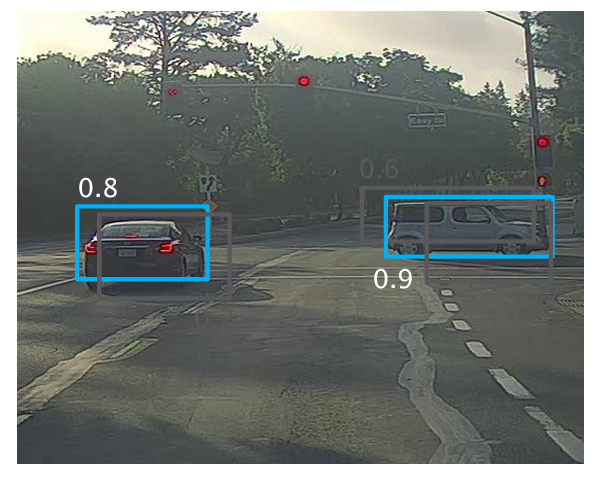
\includegraphics[scale=0.5]{img/NMS.png}
    \end{center}
    How can we choose the one that I will show onto the image? The procedure is the following, \textbf{for each class}: 
    \begin{enumerate}
        \itemsep-0.2em
        \item Discard all boxes with low probability (eg. $p_c\le{0.6}$); 
        \item Pick the box with the largest $p_c$ and discarding any remaining box with \emph{IoU}$\ge{0.5}$ having the same box output in the previous step.
    \end{enumerate}
\end{multicols}

%In the following we show an example: 

\section{Evaluating object localization and detection performance}
At this point we need a way in order to evaluate how well a prediction has been done for a certain bounding box. A metric which is used is the \textbf{Intersection over Union (IoU)}, it is a measure of the overlap between two bounding boxes: the predicted one and the \textit{ground truth} taken from the dataset. It is defined as the ratio between the intersection of the bounding boxes and the union of them.

\begin{figure}[h]
    \centering
    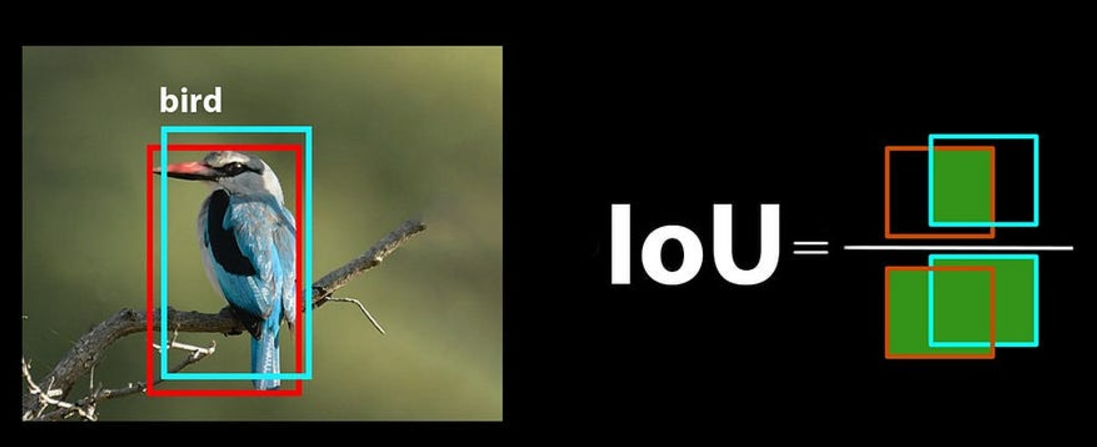
\includegraphics[scale=0.3]{img/IoU.png}
    \caption{\textbf{Intersection over Union (IoU)} definition}
\end{figure}

\noindent 
Usually we can say that a good prediction has a $
    IoU \ge 0.5
$. 

Since object detection includes a  classification task we can build a \textbf{confusion matrix} like the one we introduced in the previuous chapters, in which also/only the $IoU$ is taken into account. In particular:
\begin{itemize}
    \itemsep-0.3em
    \item A \textbf{True positive} is counted in the case that there is a correct class prediction and IoU metric greater than 0.5; 
    \item A \textbf{False positive} is counted if there is a wrong class prediction or $IoU<0.5$
    \item A \textbf{False negative} is considered in the case a certain object is not detected.
\end{itemize}
According to such assumptions we are able to compute \textit{precision} and \textit{recall} for each class and then the $F$-measure can be computed. The \textit{precision-recall curve} can be also drawn in order to select the best value for threshold depending on the user requirements.

\begin{figure}
    \centering
    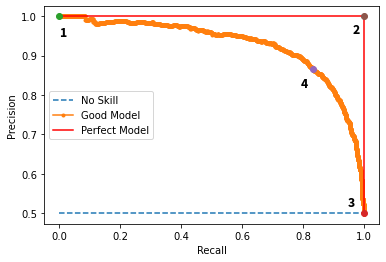
\includegraphics[scale=0.8]{img/PR_curve.png}
    \caption{\textbf{Precision-Recall Curve} for a bad, good and perfect model}
\end{figure}

A curve for each class can be drawn, and we can associate each one with another important metric: the \textit{Average precision} that is nothing but the area under the curve. The object detectors are usually ranked using the \textbf{mean Average Precision (mAP)} which is the average AP over all classes: 
\begin{equation}
    \text{mAP}=\frac{\sum_{c\in{C}}{AP_{c}}}{\vert C \vert }
\end{equation}
In some benchmarks mAP is computed at different IoU and then averaged again, this is the reason why sometimes it is denoted with $\text{mAP}^{\text{IoU}}$. 

\section{Final considerations}
Object detection architectures are not \textit{end-to-end} ones, like the models used for image classification: there are few base architectures but a lot of variations, some post-processing is required. Moreover when there are strong a-priori information are available on the target shapes the use of anchors is strongly recommended. In any case bounding boxes representation is not optimal since there can be irregular shapes, packed objects or rotated objects.

